\documentclass{article}
\usepackage[utf8]{inputenc}
\usepackage{amsmath}
\usepackage{graphicx}
\usepackage[ruled,vlined]{algorithm2e}
\usepackage{biblatex}
 
\title{Supplemental Appendix S3: \\
\large Restricted Population Models}
\author{Liu and Leighow et al.}

\begin{document}


\maketitle

\section{Introduction}
Our hypothesis that the restricted effective population size in 
Our hypothesis that the leukemic cell population hierarchy and resulting restricted effective population size in CML drives the survival of the likeliest, we sought out other pathologies that may exhibit limited effective population sizes and thus also demonstrate survival of the likeliest.

We considered three disease/treatment models: targeted therapy in the adjuvant setting; spatial heterogeneity in solid tumors where mitotitc activity is limited to the periphery; transmission bottlenecks in an infectious disease.

\section{Spatial Tumor Model}

\subsection{Introduction}
It is generally accepted that only a fraction of cells in a solid tumor are mitotically active, due to spatial heterogeneities in access to resources and space \cite{1}.  We hypothesized that this spatial structuring reduces the number of cells able to seed resistance and may give rise to survival of the likeliest.  To test this, we developed an agent-based spatial model of three-dimensional solid tumor growth and simulated a cohort of virtual tumors with two potential resistance mutations.  Mutation A is less likely but more drug resistant; mutation B is more likely but less drug resistant.  The simulation continues until eradication of all viable cells or progression due to drug resistance.

\subsection{Parameters}
For all genotypes, division rates and natural death rates were $b = 0.69$ and $d = 0.35$ /day, respectively.  Sensitive cells were killed by drug at a rate of $\alpha_S = 0.68$ /day \cite{2}.  Dead cells were cleared at a rate of $c=0.5$ /day.  When sensitive cells divided they had the potential to seed a resistance variant at a resistance mutation rate of $\mu=10^{-8}$ /division.  Mutation to either allele occurred with probabilities $\rho_A=0.2$ and $\rho_B=0.8$.  The drug kill rates for the two resistance variants were $\alpha_A=0.2\cdot(b-d)=0.068$ and $\alpha_B=0.8\cdot(b-d)=0.27$ /day.  Detection and treatment began at $M=5\times10^8$ cells.

\subsection{Model Details}

Simulations were carried out in Matlab. For computational efficiency, the base unit of our model was a homogeneous cluster of $10^6$ cells.  We scaled the mutation rate $\mu$ and size at detection $M$ appropriately.  Cell clusters occupy sites in a three-dimensional lattice, and the model is initialized with a single cluster of sensitive cells at the origin.

Events are simulated as Poisson processes as in a Gillespie algorithm.  First, the inter-event time is drawn from an exponential distribution.  Then, the specific event (division, death, clearance, or mutation) is drawn from a weighted sample.  Next, the cell $i$ that undergoes the event is selected.  In the case of cell division and death, cell $i$ is drawn from a weighted sample based on its distance from the tumor periphery.  For clearance of dead cells, cell $i$ is drawn from a uniform distribution.  Finally, the state matrices are updated to reflect the event.

\subsubsection{Cell Division}

When a division event occurs, dividing cell $i$ is chosen based on its distance from the tumor periphery.  The periphery is drawn around the tumor (Matlab's \textit{boundary} function; \textbf{Supplemental Figure 3.1} top) and the minimum distance between each viable cell and the periphery is calculated (\textbf{Supplemental Figure 3.1} bottom).

\begin{center}
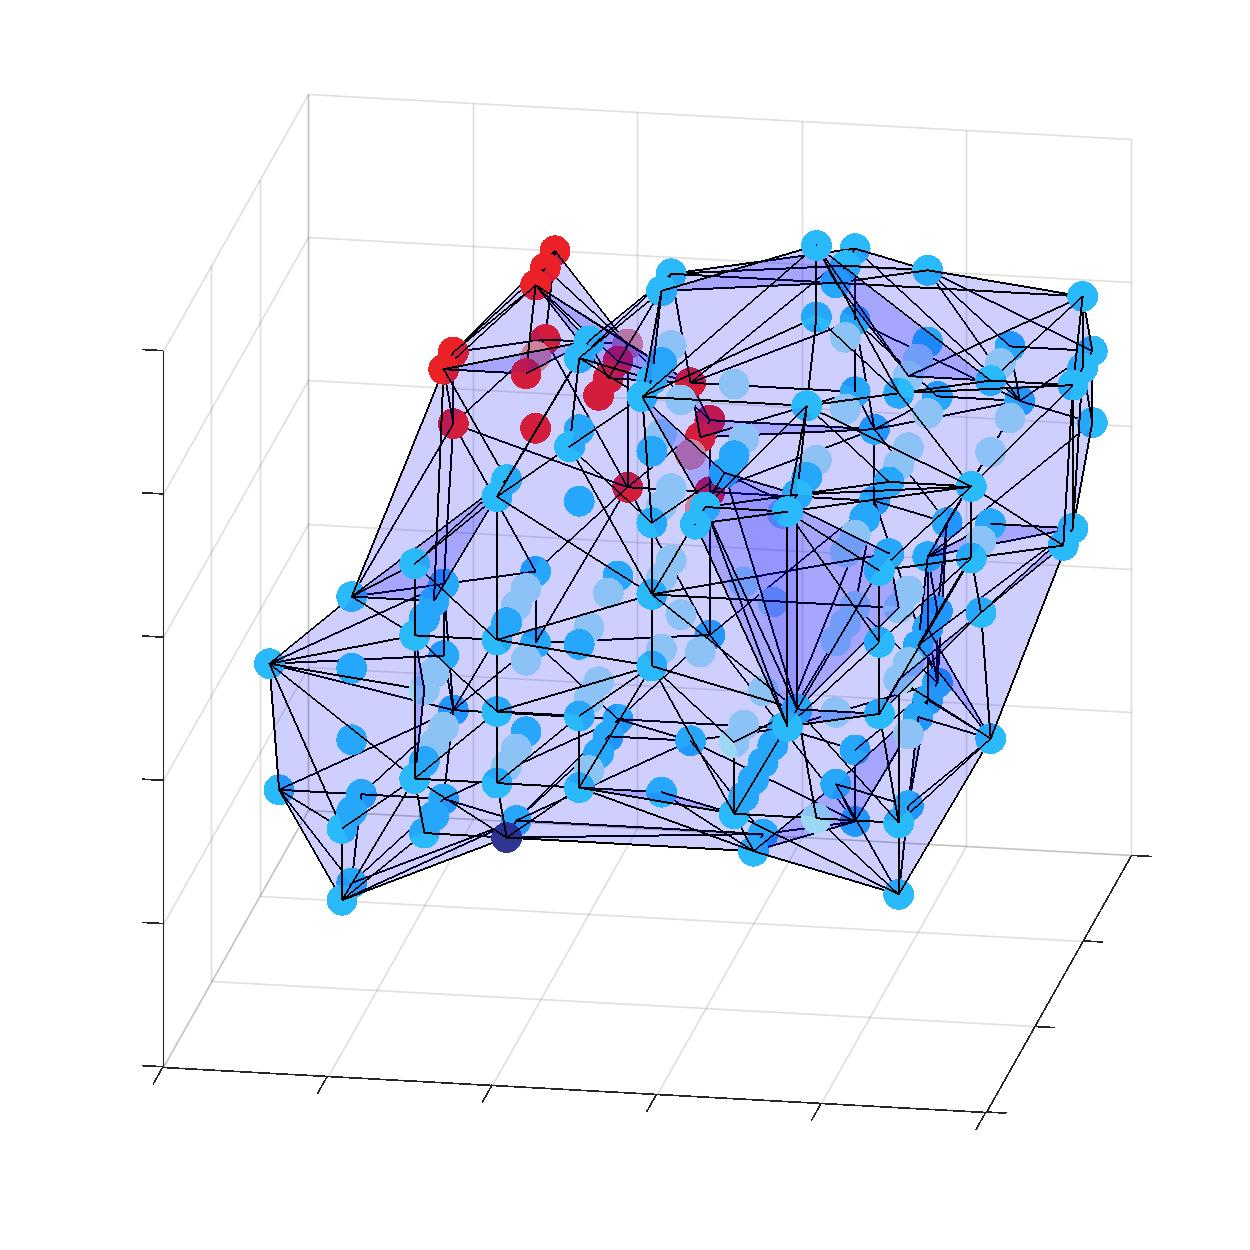
\includegraphics[width=0.65\textwidth , height=0.65\textwidth]{TumorBoundary}
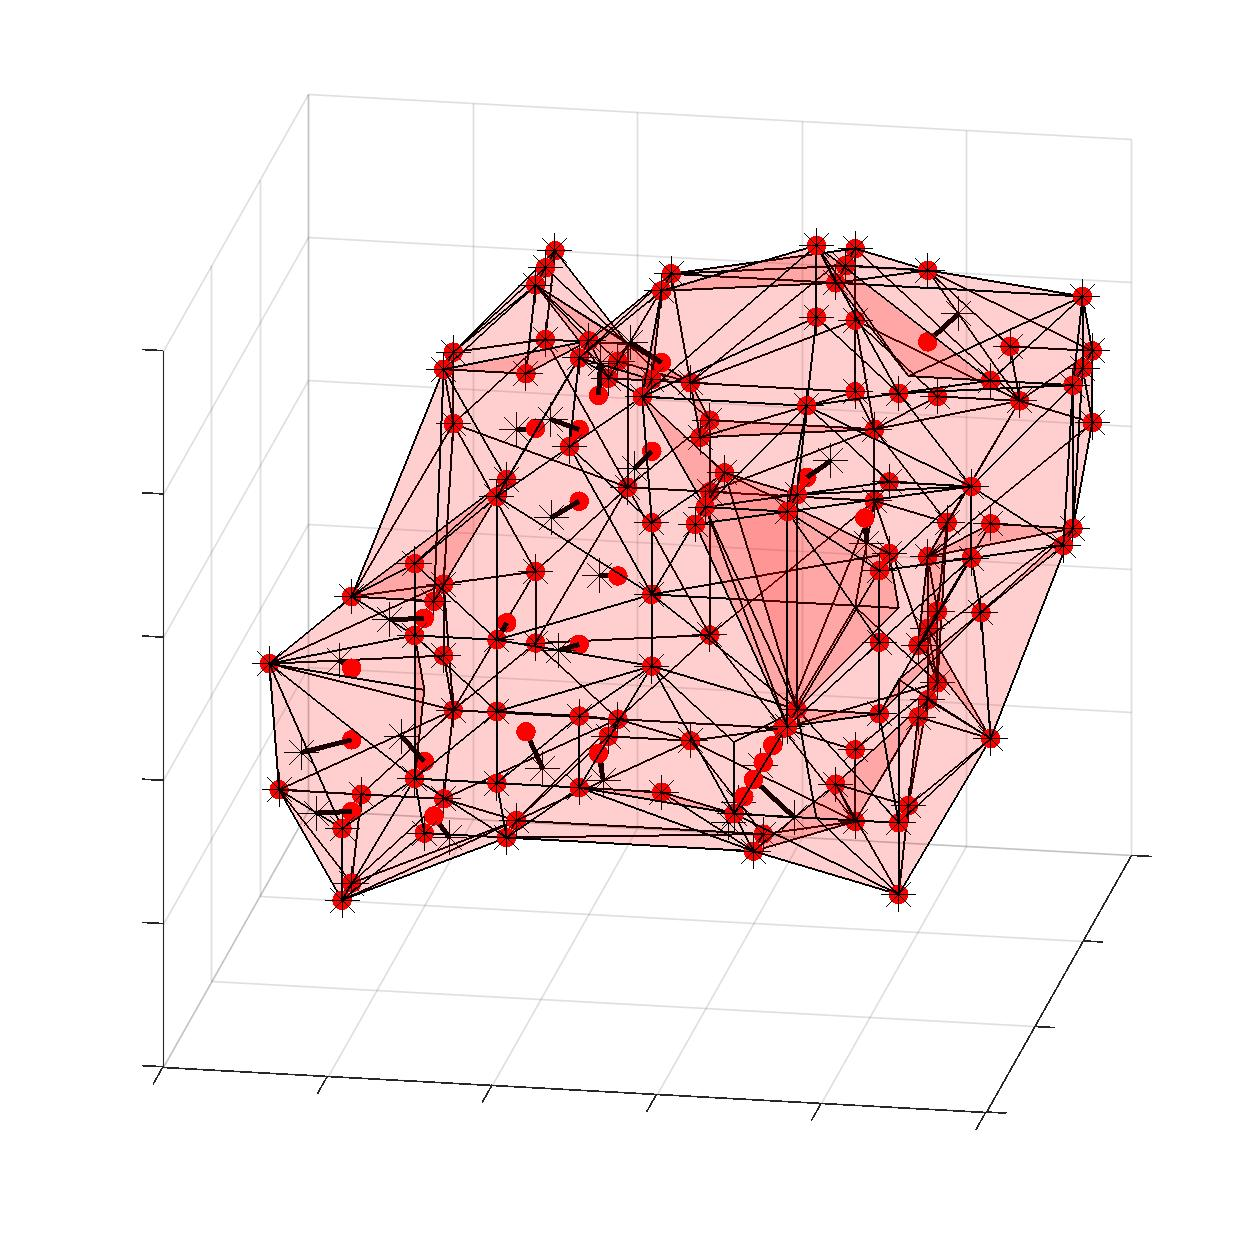
\includegraphics[width=0.65\textwidth , height=0.65\textwidth]{PeripheryDistance}

\textbf{Supplemental Figure 3.1}: \textit{Top}: Example of growing virtual tumor with viable (light blue) and necrotic (gray-blue) sensitive cells and viable (red) and necrotic (gray-red) resistant cells.  The transparent blue surface surrounding the virtual tumor is used to identify the tumor periphery.  \textit{Bottom}: Distance from the periphery (\textbf{thick} black lines) determines access to resources and drug exposure.
\end{center}

The dividing cell $i$ is then drawn from a weighted sample of the population of viable cells.  The weights for each cell are $W_i=exp(-r_i)$ where $r_i$ is the distance to the periphery.  An exponential function was chosen to reflect the limited diffusion of resources into the tumor.
 
When a sensitive cell divides it mutates to a resistant variant with probability $\mu=10^{-8}$ /division.  If a resistance mutation occurs, the resistance allele is drawn according to probabilities $\rho_A=0.2$ and $\rho_B=0.8$.

If there are unoccupied sites adjacent to cell $i$, the new cell $j$ is placed in the nearest site (by Euclidean distance; in the case of ties, the site is chosen at random).  If all of the sites adjacent to cell $i$ are occupied, the neighboring sites are scanned for free spaces, as in \cite{1}.  First, sites within $k=1$ units of $i$ are searched.  If no available sites are found, sites within $k=2$ units are searched, and so on.  Once the nearest unoccupied site (site $f$) is found, the cells in between $i$ and $f$ are pushed to make room for cell $j$.  This is done by identifying the cell $g$ adjacent to site $f$ that is closest to the line between $i$ and $f$ (distance to the line is calculated using the parallelogram definition of the cross-product, i.e. $||\vec{gf}\times\vec{if}||/||\vec{if}||$; \textbf{Supplemental Figure 3.2}).  Cell $g$ is moved to site $f$ and the process is repeated with the new vacant site where cell $g$ was previously until the vacant site is adjacent to cell $i$.  Then cell $j$ is placed in the adjacent vacant site.
 
\begin{center}
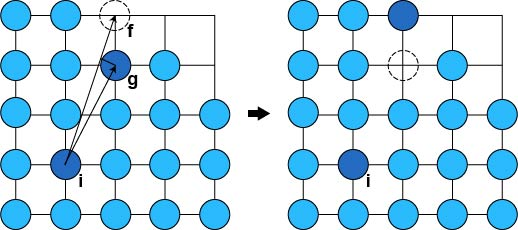
\includegraphics[width=0.75\textwidth]{Budging}

\textbf{Supplemental Figure 3.2}: Diagram of the "budging" algorithm used to make space for dividing cell clusters not on the periphery. The vacant site $f$ nearest to cell $i$ is identified, and the cell $g$ adjacent to $f$ and nearest the line between $i$ and $f$ is moved to occupy site $f$. The newly vacant site $g$ becomes the next unoccupied site for the next iteration of the algorithm until the vacant site is adjacent to $i$.
\end{center} 
 
\subsubsection{Cell Death}

When a death event occurs, the distance of viable cells from the tumor periphery is calculated as in the case of cell division.  The dying cell $i$ is drawn from a weighted sample.  In the event of a natural/necrotic cell death, the weights for each cell are $W_i=exp(r_i)$ to favor cells in the interior of the tumor.  In the event of a drug killing event, the weights for each cell are $W_i=exp(-r_i)$ to reflect greater exposure to drug at the periphery.  Upon death, the cell is no longer viable but remains part of the tumor structure until it is cleared.

\subsubsection{Dead Cell Clearance}

In the case of a dead cell clearance event, a dead cell $i$ is randomly chosen to be removed from the population.  Upon removal, the tumor fills in the unoccupied site left by the cleared cell.  The neighborhood of site $i$ is searched for the nearest unoccupied site $f$, as in the case of cell division.  The cells between $i$ and $f$ are shifted to fill in the vacancy left by clearing cell $i$ in the reverse manner as described in cell division.

\subsection{Pseudocode}

\begin{algorithm}[H]
 initialize sensitive cell cluster at the origin\;
 \While{viable cells remain and patient has not relapsed on treatment}{
  \If{number of cells exceeds detection}{
   begin treatment (update drug kill terms)\;
  }
  draw time to next event from exponential distribution\;
  draw next event from weighted sample\;
  \uIf{next event is division}{
   find distance of viable cells from tumor edge\;
   draw dividing cell $i$ from sample weighted on distance\;
   scan neighboring lattice units for unoccupied site\;
   \While{nearest unoccupied site not adjacent to cell $i$} {
    move intermediate cell into unoccupied site\;
    }
   add new cell to adjacent unoccupied site\;
   \eIf{dividing cell is sensitive and rand $<\mu$}{
    assign allele to new cell with probability $\rho$\;
   }{
    genotype of new cell matches dividing cell\;
   }
  }
  \uElseIf{next event is necrotic cell death}{
   find distance of viable cells from tumor edge\;
   select dying cell $i$ from sample weighted on distance\;
   update state of cell $i$\;
  }
  \uElseIf{next event is drug killing cell death}{
   find distance of viable cells from tumor edge\;
   select dying cell $i$ from sample weighted on distance\;
   update state of cell $i$\;
  }
  \ElseIf{next event is clearance of dead cell}{
   draw cell $i$ from population of dead cells\;
   remove cell $i$ from position and state matrices\;
   scan neighboring lattice units for unoccupied site\;
   \While{nearest free site left by cell $i$ not adjacent to unoccupied site} {
    move intermediate cell into unoccupied site left by cell $i$ or previously moved cell\;
   }
  }
  update position and state matrices\;
  update index variable\;
 } 
 \If{patient relapsed on treatment}{
  record final tumor population structure
 }
 \caption{Spatial Tumor Model Algorithm}
\end{algorithm}

\section{Adjuvant Therapy Model}

\subsection{Introduction}
Adjuvant therapy is the practice of treating a tumor in conjunction with surgery. The expectation is that surgery removes the bulk of the tumor, while the adjuvant therapy removes cancer cells that escaped resection.  We simulated a cohort of virtual patients that began with a small population of drug-sensitive cancer cells. Upon detection of the disease, a large portion of the tumor is removed and the remaining sensitive cells are treated with drug (such that their net growth rate is negative) until the sensitive population is eradicated.  Over the lifespan of the cancer, sensitive cells have the potential to seed resistant subclones (10 possible variants simulated with allele-specific resistances and biases) with positive net growth rates in the presence of drug.  The simulation continues until eradication of all cells or progression due to drug resistance, at which point the dominant resistance allele is noted.

\subsection{Parameters}
For all genotypes, division rates and natural death rates were $b = 0.14$ and $d = 0.13$ /day, respectively.  The drug kill rate for sensitive cells was $\alpha_S=0.04$ /day \cite{3}.  Allele-specific drug kill rates for resistance variants were drawn from an exponential distribution to reflect the distribution of resistance in CML (\textbf{Supplemental Figure 3.3}).

\begin{center}
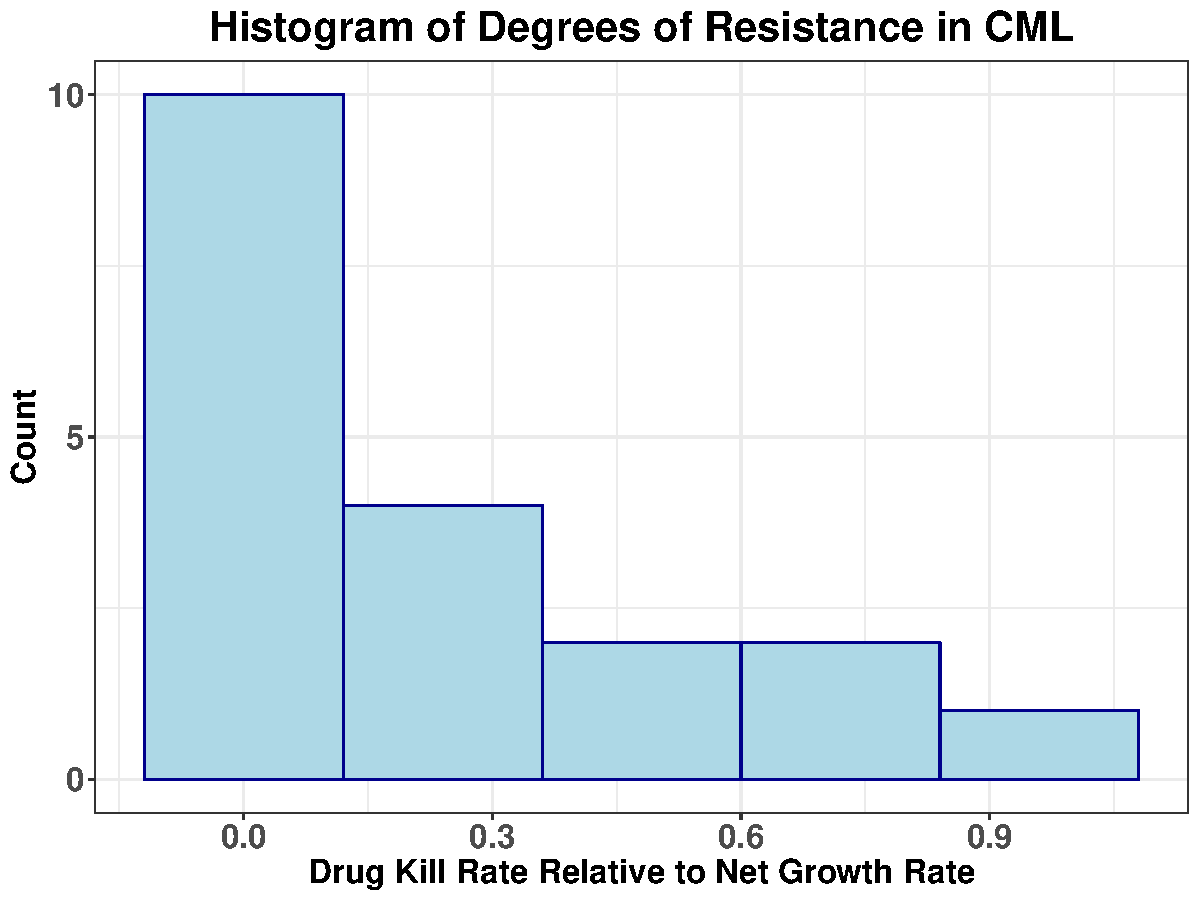
\includegraphics[width=0.75\textwidth]{CMLResistanceHistogram}

\textbf{Supplemental Figure 3.3}: Histogram of degrees of resistance in CML.  Values on the x-axis are drug kill rates for imatinib-resistant BCR-ABL variants in BaF3 cells (as calculated in \textbf{Supplemental Appendix S2}) relative to net growth rate of BaF3s.  The distribution is roughly exponential.
\end{center}

Allele-specifc mutation probabiltiies $rho_i$ were assigned from a uniform distribution and normalized to sum to unity.  The resistance mutation rate was $\mu=10^{-8}$ /division.

Tumor size upon detection/resection was variable, taking on values $M_{pre} = [10^9, 10^{10}, 10^{11}, 10^{12}]$ cells.  Likewise, the population size after resection took on values $M_{post} = [10^5, 10^6, 10^7, 10^8]$ cells.

\subsection{Model Details}
Cancer evolution was modeled stochastically as a continuous-time birth-death-mutation process.  Simulations were executed in Matlab using a Gillespie algorithm.  The propensity vector $a(\mathbf{x})$ and state change matrix $\nu$ were defined as follows:
\begin{equation}
a(\mathbf{x}) = \frac{1}{a_0}
\begin{bmatrix}
b (1-\mu) S \\
(d+\alpha_S) S \\
b \rho_1 \mu S \\
b R_1 \\
(d + \alpha_1) R_1 \\
b \rho_2 \mu S \\
b R_2 \\
\vdots
\end{bmatrix}
\end{equation}

\begin{equation}
\nu = 
\begin{bmatrix}
1 & 0 & 0 & \dots \\
-1 & 0 & 0 & \dots \\
0 & 1 & 0 & \dots \\
0 & 1 & 0 & \dots \\
0 & -1 & 0 & \dots \\
0 & 0 & 1 & \dots \\
0 & 0 & 1 & \dots \\
\vdots & \vdots & \vdots & \ddots
\end{bmatrix}
\end{equation}
Here, $a_0$ is the sum of the rates in the propensity function.

Upon detection, the sensitive population was reduced to $M_{post}$.  If any resistant cells were present prior to resection, their population size after resection was drawn from a binomial distribution with probability $p=\frac{M_{post}}{M_{pre}}$.  Before detection, $\alpha_i = 0$ for all populations.  After detection, $\alpha_i$ values were updated with appropriate drug kill terms for each variant.

\section{Transmission Bottleneck Model}

\subsection{Introduction}

Beyond cancer, pathogenic cells experience population restriction in the context of infectious disease.  In particular, transmission bottlenecks restrict the heterogeneity of the founding population when infectious pathogens are passed from one host to another.  We hypothesized that this loss of heterogeneity could favor the persistence of more likely resistance variants in the chain of transmission.  To test this, we developed an agent-based model of infectious disease.  The model considers a population of susceptible individuals and simulates within-host dynamics of infectious agents as well as between-host dynamics of transmission.  In this way, we are able to simulate \textit{de novo} resistance mutations and the spread of drug resistant variants.  

The theoretical communicable disease modeled here is treated with a first-generation drug upon detection.  Sensitive pathogens have a negative net growth rate under drug treatment, but have the potential to seed two possible resistance variants which have a positive net growth rate in the presence of the first-generation drug.  Allele A is less likely but more drug resistant; Allele B is more likely but less drug resistant.  Upon detection of the drug resistant strain, the patient is treated with a second-generation drug, to which all strains are sensitive.  Once the pathogenic population has been eradicated from a host, that individual recovers and is no longer susceptible to the disease, as in a classic SIR model \cite{4}.

\subsection{Parameters}

All pathogens replicate and die at rates of $b = 0.4$ and $d = 0.2$ /day.  Wild-type pathogens are killed by both first- and second- generation drugs at a rate of $\alpha_{S,1} = \alpha_{S,2} = 0.3$ /day.  The drug kill terms for Allele A are $\alpha_{A,1} = 0.01$ /day for the first-generation drug and $\alpha_{A,2} = 0.3$ /day for the second-generation drug.  The drug kill terms for Allele A are $\alpha_{A,1} = 0.19$ /day for the first-generation drug and $\alpha_{A,2} = 0.3$ /day for the second-generation drug.  The resistance mutation rate is $\mu=10^{-8}$, and allele-specific mutational probabilities are $\rho_A=0.25$ and $\rho_B=0.75$.  Detection and treatment initiation occur at $M=10^7$ pathogens.

There are initially $N_S=499$ susceptible individuals in the population and $N_I=1$ infected individual with 100 wild-type pathogens.  The contact rate between hosts is $\beta = 0.01$ /day, which approximates the transmission dynamics of sexually transmitted diseases \cite{5}.  The fractional bottleneck size (defined as the fraction of pathogens in an infected individual expected to be passed on to a susceptible) varies from $10^{-7} \leq \delta \leq 10^{-2}$.

\subsection{Model Details}

The model was simulated in Matlab.  Because pathogen replication and death events occur much more frequently than mutation, detection, eradication, and transmission events, within-host pathogen dynamics were modeled deterministically for the sake of computational efficiency.  

Time to detection $T_{det}$ was found using the deterministic equation:
\begin{equation}
T_{det} = \frac{1}{r} \ln(\frac{M}{M_0})
\end{equation}
where $M_0$ is the initial size of the pathogenic population.  Similarly, time to eradication $T_{erad}$ was approximated using time to population collapse of a single pathogen, with the deterministic equation:
\begin{equation}
T_{erad} = \frac{1}{r} \ln(\frac{1}{M_0})
\end{equation}
Time to mutation $T_{mut}$ is drawn from a probability density function over the time interval $[t_1,t_2]$ where $t_1$ is the current time in the simulation and $t_2$ is the time of the next change in host's state (i.e. detection and drug treatment which alters pathogen dynamics or eradication, at which point the patient has recovered and can no longer seed resistance).  The probability density function for the random variable $t_{i}$ is given from \textbf{Supplemental Appendix S1}:
\begin{equation}
f(t_{i}) = \frac{b_S \mu \rho_i r_i}{b_i} x_{S,0} e^{r_S t_{i}} \cdot \exp \big(-\frac{b_S \mu \rho_i r_i}{b_i r_S} \cdot e^{r_S t_{i}} -1 \big)
\end{equation}

Time between contact events are drawn from an exponential distribution with mean time $\lambda = \frac{\beta}{N_{tot}} N_S N_I$.  An infected individual is randomly drawn.  The structure of the founding population is given by the number of pathogens transmitted for each strain (wild-type and alleles A and B).  This quantity is drawn from a binomial distribution with number of trials $n=M_i$ and probability of success $p=\delta$.  Here $M_i$ is the number of pathogens of strain $i$ in the infected individual.  Thus, for small pathogenic population sizes (e.g. shortly after exposure or late in treatment) the expected number of transmitted pathogens is less than one.  This reflects the limited bottleneck model of transmission dynamics \cite{6} (\textbf{Supplemental Figure 3.4}).

\begin{center}
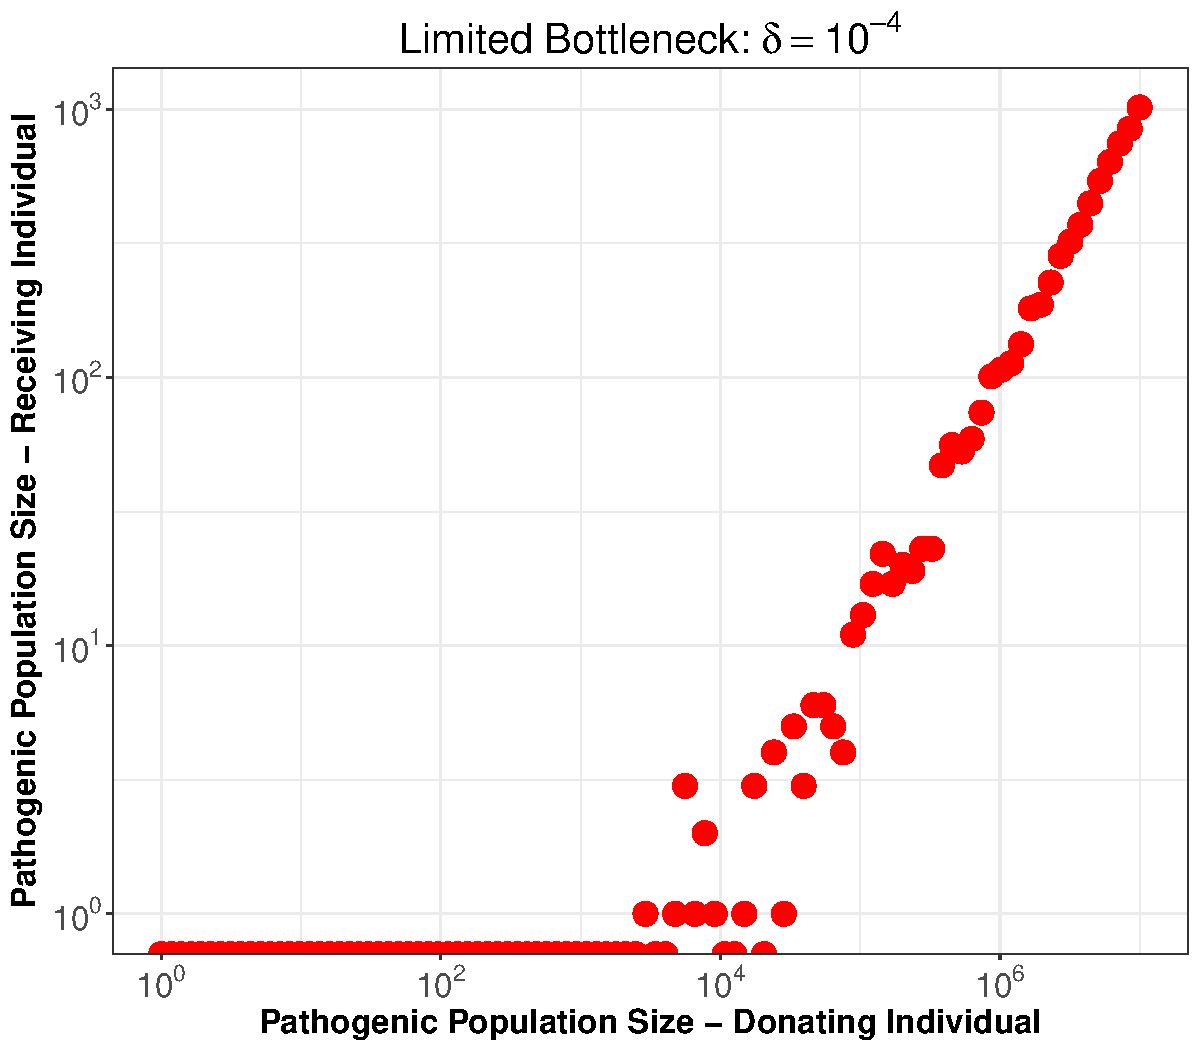
\includegraphics[width=0.75\textwidth]{LimitedBottleneck}

\textbf{Supplemental Figure 3.4}: Values on the y-axis are numbers drawn from a binomial distribution with $n =M_i=$ x-axis values and $p=\delta=10^{-4}$.
\end{center}

\subsection{Pseudocode}

\begin{algorithm}[H]
 initialize susceptibles\;
 initialize single infected individual\;
 determine times to detection and mutation in infected individual\;
 \While{number of infecteds $>0$}{
  draw time to next contact event\;
  \eIf{next contact precedes next detection/eradication/mutation}{
   inter-event time = time to contact\;
   update within host pathogen populations\;
   select infected donor and sample founding population from binomial distribution\;
   \If{founding population $>0$}{
      infect new host with founding population\;
      determine times to detection/mutation for new host\;
   }
   }{
   inter-event time = time to next detection/eradication/mutation\;
   update within host pathogen populations\;
   \uIf{next event is detection} {
      update drug (depending on detected strain)\;
      update time to mutation/detection/eradication\;
   }
   \uElseIf{next event is mutation}{   
      seed resistant population in host\;
      update time to detection\;
   }
   \ElseIf{next event is eradication}{
      remove population from host\;
      \If{all populations eradicated}{
         update status to recovered\;
         record patient history\;
      }
   }
  }
 }
 record frequency of each resistant allele\;
 \caption{Infectious Disease Model Algorithm}
\end{algorithm}


\begin{thebibliography}{9}
\bibitem{Bacevic}
K Bacevic, R Noble, A Soffar, et al. Spatial competition constrains resistance to targeted cancer therapy. \textit{Nature Communications}. 2017;8:1995.

\bibitem{Waclaw}
B Waclaw, I Bozic, ME Pittman, et al. A spatial model predicts that dispersal and cell turnover limit intratumour heterogeneity. \textit{Nature}. 2015;525(7568):261-4.

\bibitem{Bozic}
Bozic I, Reiter JG, Allen B, et al. Evolutionary dynamics of cancer in response to targeted combination therapy. \textit{Elife}. 2013;2:e00747.

\bibitem{Bjornstad}
ON Bjornstad.
\textit{Epidemics}.
Springer, Cham, Switzerland, 2018.

\bibitem{Naresh}
R Naresh, A Tripathi, D Sharma. Modelling and analysis of the spread of AIDS epidemic with immigration of HIV infectives. \textit{Mathematical and Computer Modelling}. 2009;49:880-892.

\bibitem{Abel}
S Abel, P Abel zur Wiesch, BM Davis, MK Waldor. Analysis of Bottlenecks in Experimental Models of Infection. \textit{PLOS Pathogens}. 2015;11(6)e1004823.

\end{thebibliography}

\end{document}